\section{Background} \label{sec:background}
The robotics industries association\cite{RIA} defines a robot ``a re-programmable, multi-functional, manipulator designed to move material, parts, tools or specialised devices through variable programmed motions for the performance of a variety of task''\cite{RIAdefinition}. According to that definition any device that is programmed to preform variety of tasks is classified as a robot. Most robots consist of several hardware components such as:
\begin{itemize}
	\item Physical body
	\item Actuators
	\item Sensors
	\item Controller
	\item Processor
	\item Software 
\end{itemize}
These components are commonly used when designing and developing a robot. A good design is considered to be one which best utilizes these components to reach it's goals effectively and efficiently.
\subsection{Behaviours}
Many different behaviours can be seen in day to day life. If one was trying to describe a behaviour as simply as possible, one might say a behaviour is a ``mapping of sensory inputs to a pattern of motor actions that are used to achieve a task''\cite{BehaviourDef}. The behaviours robots wish to imitate include all of the common human behaviours. Getting the robots to show a very basic version of this behaviour, such as love, would require the robot to follow nearby object in a show of attraction. Naturally, the main goal in cutting edge research is to develop these skills such that they are indistinguishable to the fully fletched human behaviours.

\subsection{E-Puck}

\begin{figure}
\centering
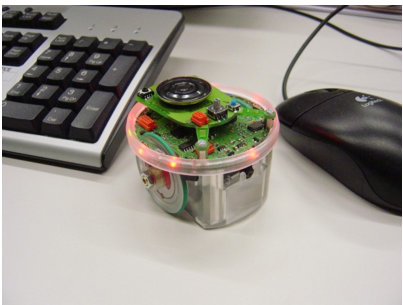
\includegraphics[width=0.7\linewidth]{figures/epcuk}
\caption{}
\label{fig:epcuk}
\end{figure}


An E-Puck\cite{epuck} is a small sized, educational robot which is designed to allow developers to code on and learn about robotics. The robot is very inexpensive, user-friendly and interactive. It was designed by Martin Stefanec from the artificial life lab of University of Graz who made all the software developed for the E-Puck open source.

It includes a wide range of sensors and actuators. Sensors include infrared-sensors which can be used to detect objects and ambient light, motors to control the movement of the robot and for communication the robot is has 8 LEDs, a speaker and bluetooth.

\subsection{HSV}

HSV stands for Hue, Saturation and value. It's a cylindrical representation of colours, starting at red in 0 degrees, green at 120 degrees and blue at 240 degrees. Using figure \ref{fig:hsv} one can recognise that the colour space's saturation is most intense in the centre of the cylinder. The saturation decides how washed out the colours appear. The final component value, which increases the higher up the cylinder the pixel value is, decides how much colour or how vibrant each colour appears.

\begin{figure}
	\centering
	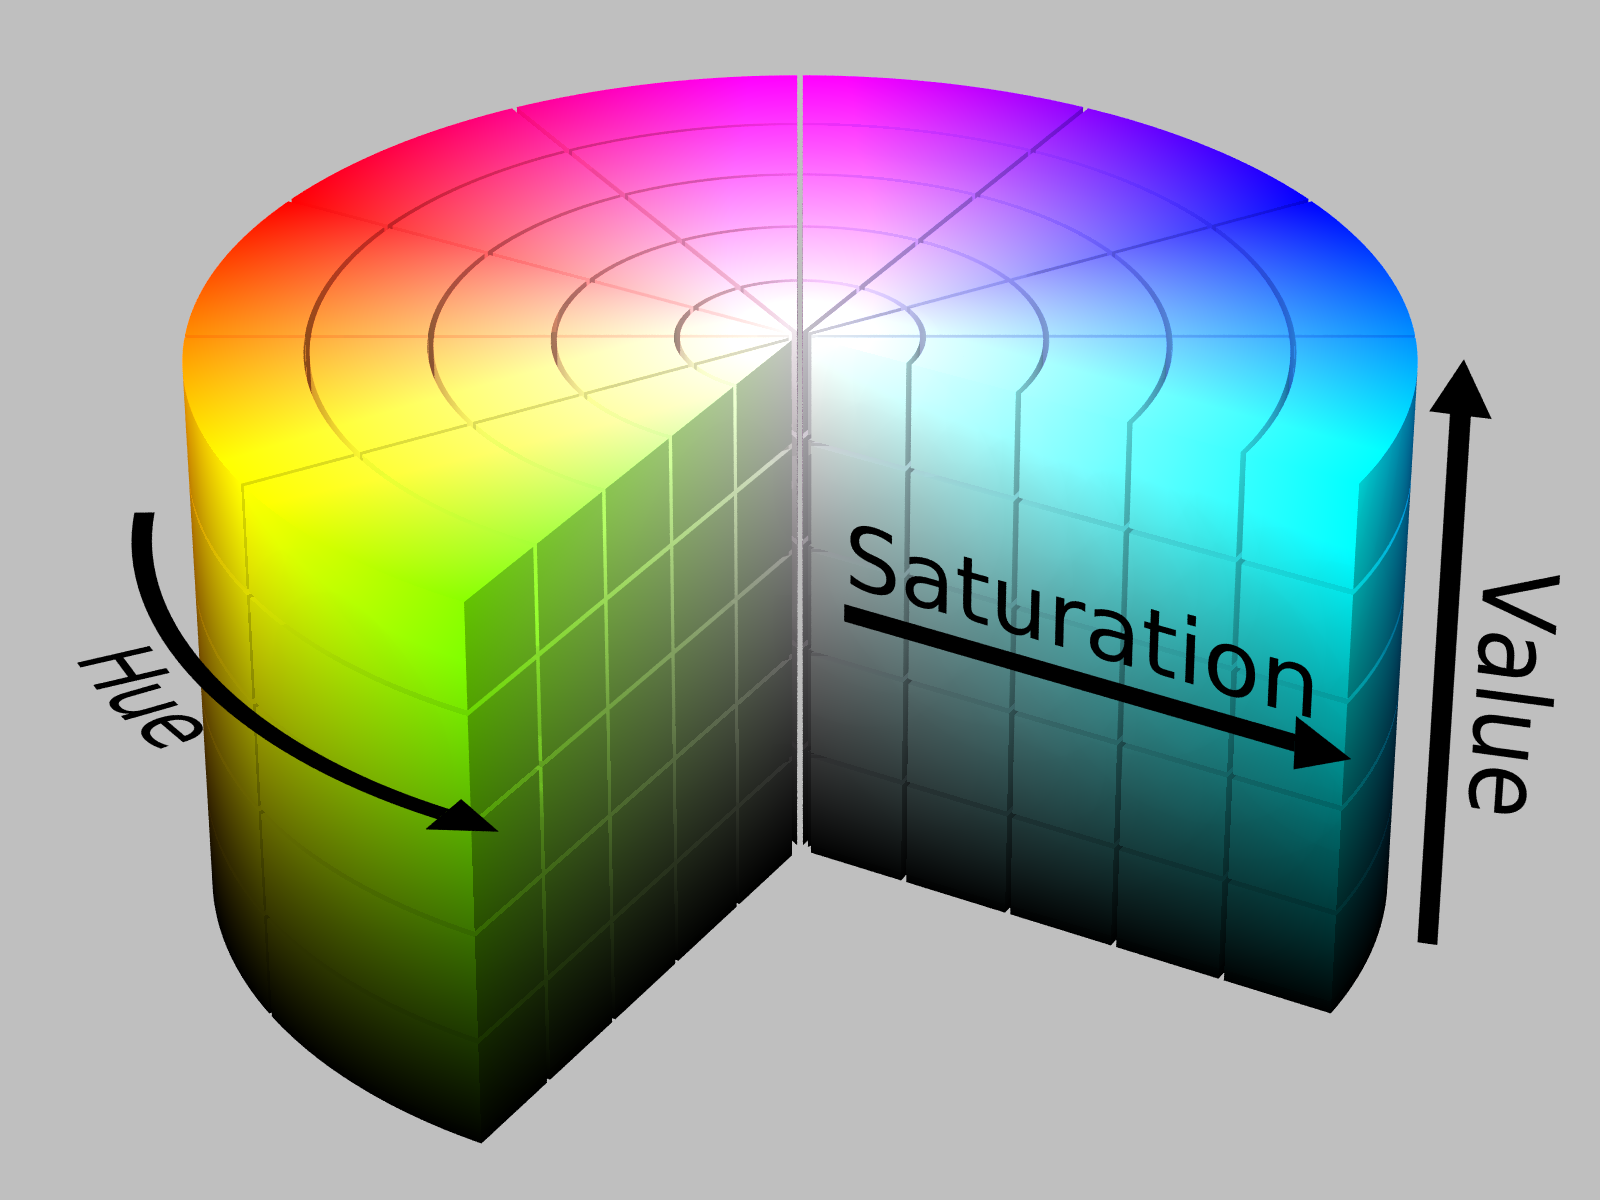
\includegraphics[width=0.7\linewidth]{figures/hsv}
	\caption{HSV Colour Space}
	\label{fig:hsv}
\end{figure}


\subsection{Skin Colour}

Skin detection in HSV tends to be more accurate than RGB. As the colour our Hue in HSV trends to be affected much less be external parameters such as ambient light or direct sunlight.

After careful research a paper found on human skin colour\cite{skinDetection}, in the HSV colour plane, found that the skin colour of the majority of people across the globe lies within the range 6\textsuperscript{o} - 38\textsuperscript{o}. The paper when on to discuss how to continue to improve the reliability of finding skin tones within an image although this is beyond the scope of this project as it would make the functions to be described much more computationally expensive. 
 